\documentclass{eegreport}

%% my usepackages
\usepackage{ltablex}
\usepackage[official]{eurosym}
\usepackage{listings}
\usepackage{subcaption}
\usepackage{amsmath, amsthm}
\usepackage{amsmath}
%\usepackage{pgfplots} gemeinsam mit matlab2tikz verwenden
	
% external files and paths
\addbibresource{Literature.bib} %% remove, if using BibTeX instead of biblatex
\graphicspath{{graphics/}}

%% general metadata:
\newcommand{\mytitle}{VU Energiemodelle und Analysen (373.011)}  %% also used for PDF metadata (hyperref)
\newcommand{\mysubject}{Protokoll Übung 3}  %% also used for PDF metadata (hyperref)
\newcommand{\myauthors}{Ivan Grubesic (01425089), Michael Kern (0935115), David Pribic (01428675), Ermin Sefer (01525021)}  %% also used for PDF metadata (hyperref)
\newcommand{\mysupervisor}{Ao.Univ.Prof. Univ.Prof. Dipl.-Ing. Dr.techn. Haas, Privatdoz. Dipl.-Ing. Dr.techn. Auer, Univ.Ass. Dipl.-Ing. Perger}  %% also used for PDF metadata (hyperref)
\newcommand{\mydate}{Mai 2020}  %% also used for PDF metadata (hyperref)

\newcommand{\mykeywords}{KEYWORDS}  %% also used for PDF metadata (hyperref)

%% this information is used only for generating the title page:
\newcommand{\myuniversity}{TU Wien} %% your university/school
\newcommand{\myinstitute}{Institut für Energiesysteme und elektrische Antriebe} %% affiliation
\newcommand{\myworkinggroup}{Energy Economics Group} %% working group
\newcommand{\mytown}{Wien} %% your home town
\newcommand{\mymonth}{Mai} %% month you are handing in
\newcommand{\myyear}{2020} %% year you are handing in

%% additional information for generic_documentation title page
\allowdisplaybreaks

\renewcommand{\thesubsubsection}{\alph{subsubsection}}
\begin{document}

\setcounter{section}{3}
\mytitlepage
\pagenumbering{Roman} 
\tableofcontents 
\pagenumbering{arabic} 

\newpage

\subsection{Fossile Erzeugung}

Es wird ein Stromversorgungssystem betrachtet. Im folgenden sind die zugehörigen Daten ersichtlich und für den ersten Abschnitt wird das abgeschlossene System ohne erneuerbare Erzeugung und Speicher bewertet. Die Gesamtkosten sollen minimal sein. \\

\begin{table}[h]
\begin{center}
\begin{tabular}{|c|c|c|c|}
\hline 
\textbf{Fossile Kraftwerke} & \textbf{Kohlekraftwerk} & \textbf{GuD-Kraftwerk} & \textbf{Gasturbine} \\ 
\hline 
Leistung [MW] & 600 & 400 & 300 \\ 
\hline 
Wirkungsgrad & 0.41 & 0.58 & 0.40 \\ 
\hline 
Brennstoffkosten [EUR/$MWh_{prim}$] & 10 & 25 & • \\ 
\hline 
$CO_2$-Emissionsfaktoren [t$CO_2$/$MWh_{prim}$] & 0.35 & 0.2 & • \\ 
\hline 
\end{tabular} 

\end{center}
\caption{Angabe Aufgabe 3.1}
\label{eos}
\end{table}
\newpage
\subsubsection{Kostenminimaler Kraftwerkseinsatz, Gesamtkosten und Emissionen}

In der nachfolgenden Tabelle ist die kostenminimale Kraftwerksnutzung (es ist jeweils die Leistung in MW angegeben) ersichtlich:

\begin{table}[h]
\begin{center}
\begin{tabular}{|c|c|c|c|}
\hline 
\textbf{Stunde} & \textbf{Kohle} & \textbf{GuD} & \textbf{Gasturbine} \\ 
\hline 
1 & 600 & 0 & 0 \\ 
\hline 
2 & 560 & 0 & 0 \\ 
\hline 
3 & 540 & 0 & 0 \\ 
\hline 
4 & 530 & 0 & 0 \\ 
\hline 
5 & 520 & 0 & 0 \\ 
\hline 
6 & 560 & 0 & 0 \\ 
\hline 
7 & 600 & 60 & 0 \\ 
\hline 
8 & 600 & 240 & 0 \\ 
\hline 
9 & 600 & 340 & 0 \\ 
\hline 
10 & 600 & 380 & 0 \\ 
\hline 
11 & 600 & 400 & 40 \\ 
\hline 
12 & 600 & 400 & 100 \\ 
\hline 
13 & 600 & 400 & 70 \\ 
\hline 
14 & 600 & 400 & 50 \\ 
\hline 
15 & 600 & 400 & 40 \\ 
\hline 
16 & 600 & 400 & 30 \\ 
\hline 
17 & 600 & 360 & 0 \\ 
\hline 
18 & 600 & 240 & 0 \\ 
\hline 
19 & 600 & 220 & 0 \\ 
\hline 
20 & 600 & 140 & 0 \\ 
\hline 
21 & 600 & 140 & 0 \\ 
\hline 
22 & 600 & 120 & 0 \\ 
\hline 
23 & 600 & 100 & 0 \\ 
\hline 
24 & 600 & 40 & 0 \\ 
\hline 
\end{tabular} 
\end{center}
\caption{Kostenminimaler Kraftwerkseinsatz Aufgabe 3.1}
\label{eosa}
\end{table}
Hier kann man erkennen das zuerst das Kohlekraftwerk bis zum Leistungsgrenzwert ausgenutzt wird. Erst dann folgen abschnittsweise die anderen Kraftwerke, in Abhängigkeit der Höhe der Grenzkosten.

Die Gesamtkosten für die Stromproduktion für diesen Tag belaufen sich daher auf 667815EUR.

Für die Stromproduktion an diesem Tag fallen 13858 Tonnen t$CO_2$ an.

\newpage
\subsubsection{Grafische Darstellung}


\myfig{punkt3.1}
       {width=1.0\textwidth}
       {optimale Nutzung des Kraftwerkparks in Abhängigkeit der Tageszeit}
       {optimale Nutzung des Kraftwerkparks in Abhängigkeit der Tageszeit}
       {optimale Nutzung des Kraftwerkparks in Abhängigkeit der Tageszeit}
       {h!}  

\newpage
\subsubsection{Schattenvariable}

Mit dem Befehl dual(Constraints(25)) werden die Schattenvariablen der 25. Bedingung ausgegeben. Diese stellen den negierten Wert der kurzfristigen Grenzkosten zu jeder Stunde dar. Nachfolgend sind die bereits invertierten Werte als Grenzkosten zu jeder Stunde in einer Tabelle dargestellt


\begin{table}[h]
\begin{center}
\begin{tabular}{|c|c|}
\hline 
\textbf{Stunde} & \textbf{Grenzkosten in EUR/MWh} \\ 
\hline 
1 & 30.3659 \\ 
\hline 
2 & 30.3659 \\ 
\hline 
3 & 30.3659 \\ 
\hline 
4 & 30.3659 \\ 
\hline 
5 & 30.3659 \\ 
\hline 
6 & 30.3659 \\ 
\hline 
7 & 45.5172 \\ 
\hline 
8 & 45.5172 \\ 
\hline 
9 & 45.5172 \\ 
\hline 
10 & 45.5172 \\ 
\hline 
11 & 66,0000 \\ 
\hline 
12 & 66,0000 \\ 
\hline 
13 & 66,0000 \\ 
\hline 
14 & 66,0000 \\ 
\hline 
15 & 66,0000 \\ 
\hline 
16 & 66,0000 \\ 
\hline 
17 & 45,5172 \\ 
\hline 
18 & 45,5172 \\ 
\hline 
19 & 45,5172 \\ 
\hline 
20 & 45,5172 \\ 
\hline 
21 & 45,5172 \\ 
\hline 
22 & 45,5172 \\ 
\hline 
23 & 45,5172 \\ 
\hline 
24 & 45,5172 \\ 
\hline 
\end{tabular} 
\end{center}
\caption{Kurzfristige Grenzkosten - Tagesübersicht}
\label{eosb}
\end{table}


\subsubsection{Stündlicher Strompreis bei optimalem Wettbewerb}
Der stündliche Strompreis unter optimalem Wettbewerb entspricht gerade den kurzfristigen Grenzkosten. Es werden immer die Stromerzeugungskosten des teuersten Kraftwerks herangezogen (Merit-Order).


\newpage
\subsection{Erneuerbare Erzeugung}
In dieser Aufgabe sollen zusätzlich die erneuerbaren Energieerzeuger Photovoltaik und
Windkraftanlage berücksichtigt werden. In nachfolgender Tabelle sind die gegebenen Werte angegeben.

\begin{table}[h]
\begin{center}
\begin{tabular}{|c|c|c|}
\hline 
• & \textbf{Wind}  & \textbf{Photovoltaik} \\ 
\hline 
Leistung [MW] & 500 & 100 \\ 
\hline 
Wirkungsgrad & 1 & 1 \\ 
\hline 
Einspeisevergütung [EUR/MWh] & 70 & 100 \\ 
\hline 
$CO_2$-Emissionsfaktoren [t$CO_2$/$MWh_{prim}$] & 0 & 0 \\ 
\hline 
\end{tabular} 
\end{center}
\caption{Angabe Aufgabe 3.2}
\label{eosc}
\end{table}
\newpage
\subsubsection{Kostenminimaler Kraftwerkseinsatz, Gesamtkosten und Emissionen}

\begin{table}[h]
\begin{center}
\begin{tabular}{|c|c|c|c|c|c|}
\hline 
\textbf{Stunde} & \textbf{Kohle} & \textbf{GuD} & \textbf{Gasturbine} & \textbf{Wind} & \textbf{PV} \\ 
\hline 
1 & 333,88 & 0,00 & 0,00 & 266,12 & 0,00 \\ 
\hline 
2 & 337,20 & 0,00 & 0,00 & 222,80 & 0,00 \\ 
\hline 
3 & 330,23 & 0,00 & 0,00 & 209,77 & 0,00 \\ 
\hline 
4 & 338,14 & 0,00 & 0,00 & 191,86 & 0,00 \\ 
\hline 
5 & 364,09 & 0,00 & 0,00 & 153,91 & 2,00 \\ 
\hline 
6 & 365,84 & 0,00 & 0,00 & 186,16 & 8,00 \\ 
\hline 
7 & 467,83 & 0,00 & 0,00 & 171,17 & 21,00 \\ 
\hline 
8 & 600,00 & 36,13 & 0,00 & 162,87 & 41,00 \\ 
\hline 
9 & 600,00 & 47,92 & 0,00 & 232,08 & 60,00 \\ 
\hline 
10 & 600,00 & 55,19 & 0,00 & 250,81 & 74,00 \\ 
\hline 
11 & 600,00 & 70,00 & 0,00 & 289,00 & 81,00 \\ 
\hline 
12 & 600,00 & 120,00 & 0,00 & 300,00 & 80,00 \\ 
\hline 
13 & 600,00 & 152,00 & 0,00 & 243,00 & 75,00 \\ 
\hline 
14 & 600,00 & 184,00 & 0,00 & 200,00 & 66,00 \\ 
\hline 
15 & 600,00 & 271,33 & 0,00 & 116,67 & 52,00 \\ 
\hline 
16 & 600,00 & 319,00 & 0,00 & 75,00 & 36,00 \\ 
\hline 
17 & 600,00 & 248,63 & 0,00 & 91,37 & 20,00 \\ 
\hline 
18 & 600,00 & 112,62 & 0,00 & 119,38 & 8,00 \\ 
\hline 
19 & 600,00 & 65,39 & 0,00 & 152,61 & 2,00 \\ 
\hline 
20 & 595,21 & 0,00 & 0,00 & 144,79 & 0,00 \\ 
\hline 
21 & 593,09 & 0,00 & 0,00 & 146,91 & 0,00 \\ 
\hline 
22 & 516,58 & 0,00 & 0,00 & 203,42 & 0,00 \\ 
\hline 
23 & 456,68 & 0,00 & 0,00 & 243,32 & 0,00 \\ 
\hline 
24 & 371,92 & 0,00 & 0,00 & 268,08 & 0,00 \\ 
\hline 
\end{tabular} 
\end{center}
\caption{Kostenminimaler Kraftwerkseinsatz mit erneuerbarer Energiekraftwerke ohne Speicher}
\label{eosd}
\end{table}
Durch den Priority-Feed-In werden die erneuerbaren Energiekraftwerke als erstes voll genutzt und erst danach die, von den Grenzkosten her, nächst teureren Kraftwerke. In unserem speziellen Fall kommt die Gasturbine überhaupt nicht mehr zum Einsatz.
Die Gesamtkosten für die Stromproduktion für diesen Tag belaufen sich daher auf 61704EUR unter Berücksichtigung der Einspeisevergütung. 
Ohne Einspeisevergütung ergeben sich die Gesamtkosten zu 449180EUR.
Für die Stromproduktion an diesem Tag fallen 11055 Tonnen $CO_2$ an.


\newpage
\subsubsection{Grafische Darstellung}

\myfig{punkt3.2}
       {width=1.0\textwidth}
       {optimale Nutzung des Kraftwerkparks in Abhängigkeit der Tageszeit}
       {optimale Nutzung des Kraftwerkparks in Abhängigkeit der Tageszeit}
       {optimale Nutzung des Kraftwerkparks in Abhängigkeit der Tageszeit}
       {h!} 

\newpage
\subsubsection{Stündlicher Strompreis}
\begin{table}[h]
\begin{center}
\begin{tabular}{|c|c|}
\hline 
\textbf{Stunde} & \textbf{Kosten} \\ 
\hline 
1 & 30,37 \\ 
\hline 
2 & 30,37 \\ 
\hline 
3 & 30,37 \\ 
\hline 
4 & 30,37 \\ 
\hline 
5 & 30,37 \\ 
\hline 
6 & 30,37 \\ 
\hline 
7 & 45,52 \\ 
\hline 
8 & 45,52 \\ 
\hline 
9 & 45,52 \\ 
\hline 
10 & 45,52 \\ 
\hline 
11 & 45,52 \\ 
\hline 
12 & 45,52 \\ 
\hline 
13 & 45,52 \\ 
\hline 
14 & 45,52 \\ 
\hline 
15 & 45,52 \\ 
\hline 
16 & 45,52 \\ 
\hline 
17 & 45,52 \\ 
\hline 
18 & 45,52 \\ 
\hline 
19 & 45,52 \\ 
\hline 
20 & 30,37 \\ 
\hline 
21 & 30,37 \\ 
\hline 
22 & 30,37 \\ 
\hline 
23 & 30,37 \\ 
\hline 
24 & 30,37 \\ 
\hline 
\end{tabular} 
\end{center}
\caption{Stündlicher Strompreis}
\label{ab}
\end{table}


\newpage
\subsection{Speicher}

Es wird weiterhin das Stromversorgungssytem betrachtet hinzu kommt in diesem Unterpunkt die Implementierung eines Speichers. Der Speicher fasst eine Energiemenge von 600MWh.
Für unsere Gruppe wurden folgende Leistungswerte für das Turbinieren und Pumpen gewählt:
Turbinieren und Pumpen: 200MW

\subsubsection{Kostenminimaler Kraftwerkseinsatz, Gesamtkosten und Emissionen}


\begin{table}[h]
\begin{center}
\begin{tabular}{|c|c|c|c|c|c|c|c|}
\hline 
\textbf{Stunde} & \textbf{Kohle}  & \textbf{GuD} & \textbf{Gasturbine} & \textbf{Wind} & \textbf{PV} & \textbf{Turbinieren} & \textbf{Pumpen}  \\
\hline 
1      & 333,88 & 0,00   & 0,00       & 266,12 & 0,00  & 0,00        & 0,00    \\
\hline 
2      & 337,20 & 0,00   & 0,00       & 222,80 & 0,00  & 0,00        & 0,00    \\
\hline 
3      & 530,23 & 0,00   & 0,00       & 209,77 & 0,00  & 0,00        & -200,00 \\
\hline 
4      & 338,14 & 0,00   & 0,00       & 191,86 & 0,00  & 0,00        & 0,00    \\
\hline 
5      & 498,59 & 0,00   & 0,00       & 153,91 & 2,00  & 0,00        & -134,49 \\
\hline 
6      & 565,84 & 0,00   & 0,00       & 186,16 & 8,00  & 0,00        & -200,00 \\
\hline 
7      & 600,00 & 0,00   & 0,00       & 171,17 & 21,00 & 0,00        & -132,17 \\
\hline 
8      & 600,00 & 36,13  & 0,00       & 162,87 & 41,00 & 0,00        & 0,00    \\
\hline 
9      & 600,00 & 47,92  & 0,00       & 232,08 & 60,00 & 0,00        & 0,00    \\
\hline 
10     & 600,00 & 55,19  & 0,00       & 250,81 & 74,00 & 0,00        & 0,00    \\
\hline 
11     & 600,00 & 70,00  & 0,00       & 289,00 & 81,00 & 0,00        & 0,00    \\
\hline 
12     & 600,00 & 120,00 & 0,00       & 300,00 & 80,00 & 0,00        & 0,00    \\
\hline 
13     & 600,00 & 152,00 & 0,00       & 243,00 & 75,00 & 0,00        & 0,00    \\
\hline 
14     & 600,00 & 44,00  & 0,00       & 200,00 & 66,00 & 140,00      & 0,00    \\
\hline 
15     & 600,00 & 71,33  & 0,00       & 116,67 & 52,00 & 200,00      & 0,00    \\
\hline 
16     & 600,00 & 119,00 & 0,00       & 75,00  & 36,00 & 200,00      & 0,00    \\
\hline 
17     & 600,00 & 248,63 & 0,00       & 91,37  & 20,00 & 0,00        & 0,00    \\
\hline 
18     & 600,00 & 112,62 & 0,00       & 119,38 & 8,00  & 0,00        & 0,00    \\
\hline 
19     & 600,00 & 65,39  & 0,00       & 152,61 & 2,00  & 0,00        & 0,00    \\
\hline 
20     & 595,21 & 0,00   & 0,00       & 144,79 & 0,00  & 0,00        & 0,00    \\
\hline 
21     & 593,09 & 0,00   & 0,00       & 146,91 & 0,00  & 0,00        & 0,00    \\
\hline 
22     & 516,58 & 0,00   & 0,00       & 203,42 & 0,00  & 0,00        & 0,00    \\
\hline 
23     & 456,68 & 0,00   & 0,00       & 243,32 & 0,00  & 0,00        & 0,00    \\
\hline 
24     & 371,92 & 0,00   & 0,00       & 268,08 & 0,00  & 0,00        & 0,00   \\
\hline 
\end{tabular}
\end{center}
\caption{Kostenminimaler Kraftwerkseinsatz mit erneuerbarer Energiekraftwerke und Speicher}
\label{ac}
\end{table}

Die Gesamtkosten für die Stromproduktion für diesen Tag belaufen sich auf 57368EUR unter Berücksichtigung der Einspeisevergütung. 
Ohne Einspeisevergütung ergeben sich die Gesamtkosten zu 444845EUR.
Für die Stromproduktion an diesem Tag fallen 11438 Tonnen $CO_2$ an. 
Nachfolgend wieder die grafische Darstellung der Situation.

\myfig{punkt3.3}
       {width=1.0\textwidth}
       {optimale Nutzung des Kraftwerkparks in Abhängigkeit der Tageszeit}
       {optimale Nutzung des Kraftwerkparks in Abhängigkeit der Tageszeit}
       {optimale Nutzung des Kraftwerkparks in Abhängigkeit der Tageszeit}
       {h!} 

\subsubsection{Mathematische Formulierung}


Der Optimierungsalhorithmus wird versuchenden Energiespeicher in frühen Stunden aufzufüllen und zu Lastspitz-Zeiten zu leeren um 
den Kraftwerkseinsatz von GuD weiter zu senken.

\begin{equation}
TotalCosts = \sum\nolimits_{i=1}^7 P_i \cdot MarginalCosts;
\end{equation}


Die Nebenbedingungen:

\begin{equation}
0 \leq E_{prim}  \leq max(E_t)
\end{equation}

\begin{equation}
0 \leq P_{pump}  \leq max(P_{pump})
\end{equation}

\begin{equation}
0 \leq P_{turbinieren}  \leq max(P_{turbinieren})
\end{equation}

Der Energiespeicher soll zum Anfangszeitpunkt (hier Stunde 1) und Endzeitpunkt (hier Stunde 24) leer sein:
\begin{equation}
E_1=E_{24}=0
\end{equation}

\begin{equation}
E_t= E_{t-1} + P_{pump,t} \cdot \eta - P_{turbinieren,t}/ \eta
\end{equation}

 
\subsubsection{Veränderung der Emissionen durch Speichernutzung}
Die Speichernutzung wirkt sich negativ auf den $CO_2$-Ausstoß aus, da hier nicht Emissionsminimal, sondern (bis auf den Priority-Feed-In) Kostenminimal optimiert wird. Der zusätzliche Emissionsausstoß entsteht durch das aufladen des Speichers mit Hilfe des günstigen Kohlekraftwerks in den Frühstunden.
Es können mit einem Speicher somit Kosten eingespart werden, ohne zusätzliche Regulierungen würden aber gerade die Kohlekraftwerke noch mehr davon profitieren. 
Aus Umweltbewusster Sicht ist dies nicht empfehlenswert.


\subsubsection{Änderung stündlicher Strompreise}
Im Vergleich zur Aufgabe 3.2 haben sich die Strompreise hier nicht verändert. Sie bleiben trotz Speicher gleich.


\subsubsection{Einsatzkostenvergleich der 3 Modelle}
Nachfolgend sind die Gesamtkosten der 3 unterschiedlichen Modelle (Aufgaben 3.1 bis 3.3):

\begin{table}[h]
\begin{center}
\begin{tabular}{|c|c|c|}
\hline 
Modell & Gesamtkosten(ohne Vergütung) & Emission (in Tonnen $CO_2$) \\ 
\hline 
3.1 & 667815 EUR & 13858 EUR \\ 
\hline 
3.2 & 449180 EUR & 11055 EUR \\ 
\hline 
3.3 & 444845 EUR & 11438 EUR \\ 
\hline 
\end{tabular} 
\end{center}
\caption{Einsatzkostenvergleich der 3 Modelle}
\label{ad}
\end{table}

\newpage

\subsection{Kosten vs. Emissionen}
\subsubsection{Minimale Gesamtemissionen}
Das Modell wurde in MATLAB optimisiert und die Werte findet man in folgenden Tabellen.

\begin{table}[h]
\begin{center}
\begin{tabular}{|c|c|c|c|}
\hline
\multicolumn{4}{|c|}{\textbf{ohne Speicher}} \\
\hline 
\multicolumn{2}{|c|}{\textbf{Kostenminimal}} & \multicolumn{2}{|c|}{\textbf{Emissionsminimal}} \\ 
\hline 
Gesamtkosten & 61704 EUR & Gesamtkosten & 318914 EUR \\ 
\hline 
Gesamtemission & 11055 t$CO_2$ & Gesamtemission & 5793 t$CO_2$ \\ 
\hline 
\end{tabular} 
\end{center}
\caption{Werte ohne Speicher}
\label{wos}
\end{table}


\begin{table}[h]
\begin{center}
\begin{tabular}{|c|c|c|c|}
\hline
\multicolumn{4}{|c|}{\textbf{mit Speicher}} \\
\hline 
\multicolumn{2}{|c|}{\textbf{Kostenminimal}} & \multicolumn{2}{|c|}{\textbf{Emissionsminimal}} \\ 
\hline 
Gesamtkosten & 57368 EUR & Gesamtkosten & 341099 EUR \\ 
\hline 
Gesamtemission & 11438 t$CO_2$ & Gesamtemission & 5624 t$CO_2$ \\ 
\hline 
\end{tabular} 
\end{center}
\caption{Werte mit Speicher}
\label{wms}
\end{table}		

Die Gesamtkosten steigen bei den beiden emissionsminimalen Systemen dramatisch an, da auf die Wirtschaftlichkeit verzichtet wird und der Naturschutz im Vordergrund gestellt wird. Wobei mit dem Speichersystem in beiden Fällen mehr optimiert wird, d.h. die Gesamtkosten beim kostenminimalen System werden noch reduziert und die Emissionen beim emissionsminimalen System werden noch weniger. 

\subsubsection{Graphische Darstellung}
Die graphische Darstellung der obigen Tabellen und Interpretation findet man in  diesem Unterpunkt. Es ist ersichtlich das die Merit Order Kurve nach rechts verschieben will wenn man den Speicher im Einsatz nimmt (EET Einfluss).

\begin{figure}
\begin{subfigure}{.5\textwidth}
  \centering
  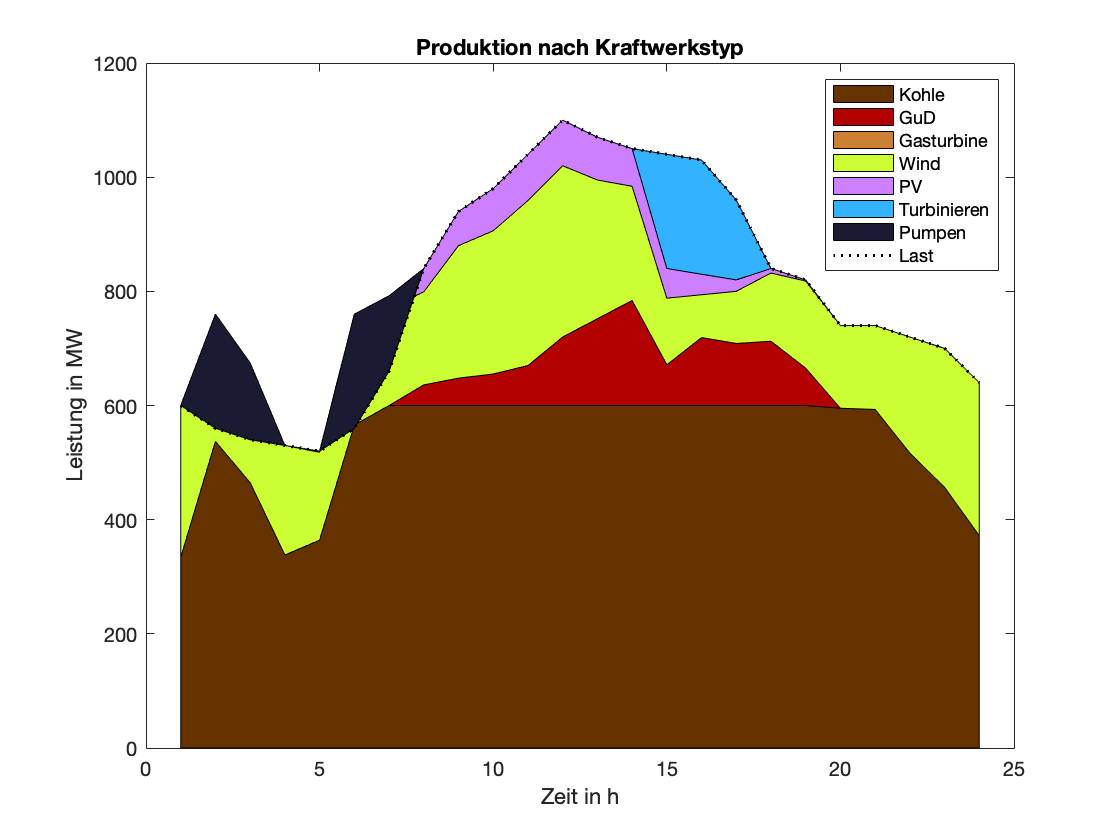
\includegraphics[width=1\linewidth]{graphics/Aufgabe_3_4_b_mit_Speicher_Kosten}
  \caption{mit Speicher System}
  \label{fig:mssks}
\end{subfigure}%
\begin{subfigure}{.5\textwidth}
  \centering
  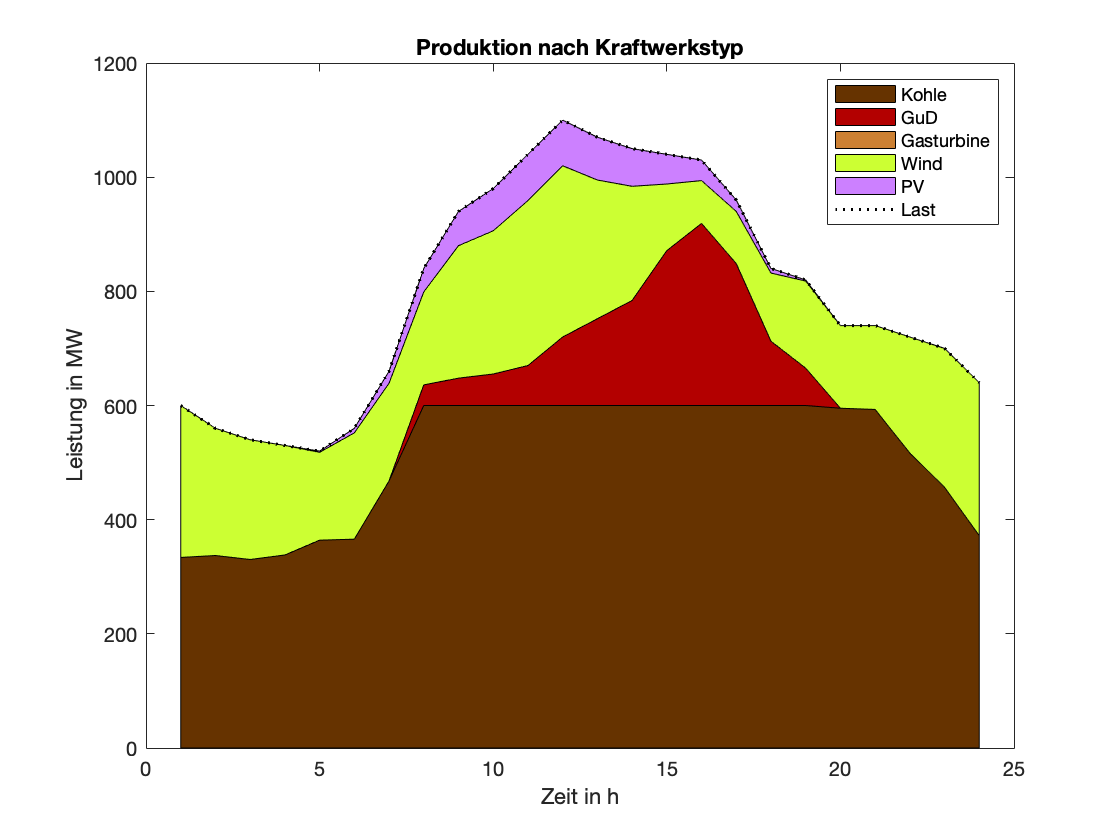
\includegraphics[width=1\linewidth]{graphics/Aufgabe_3_4_b_ohne_Speicher_Kosten}
  \caption{ohne Speicher System}
  \label{fig:ossks}
\end{subfigure}
\caption{Kostenminimale Systeme}
\label{fig:ks}
\end{figure}

\begin{figure}
\begin{subfigure}{.5\textwidth}
  \centering
  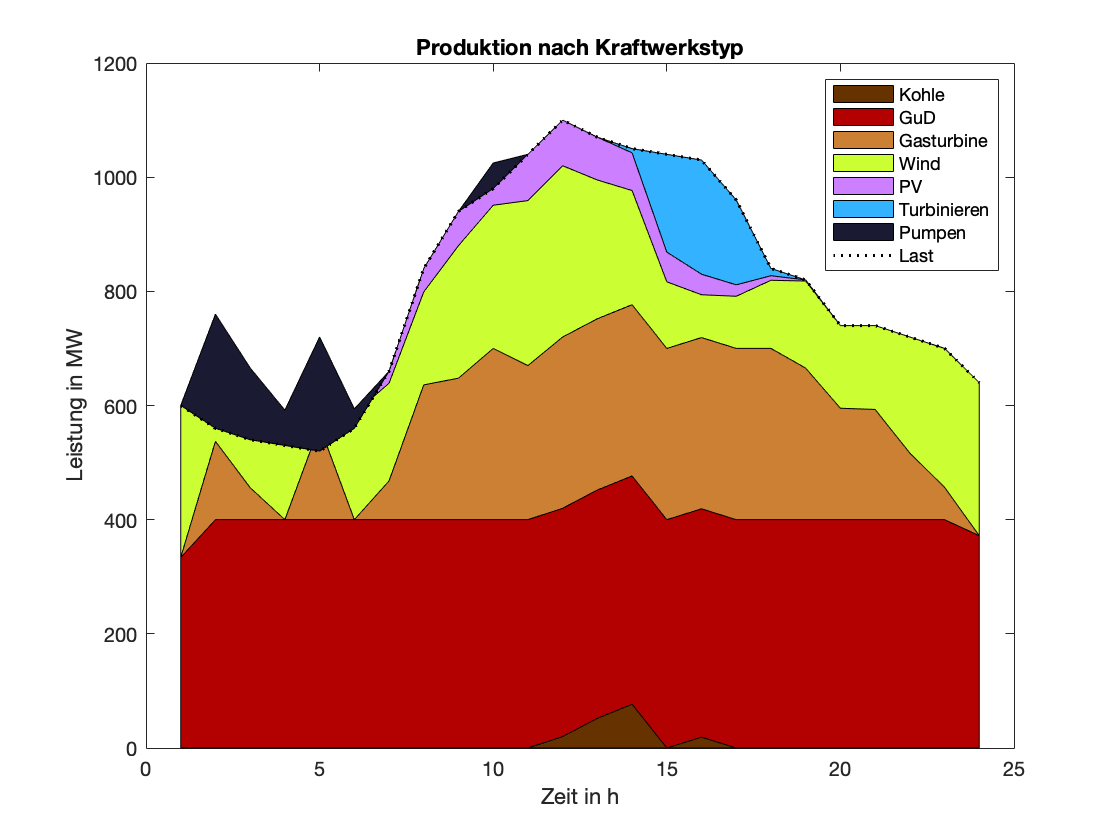
\includegraphics[width=1\linewidth]{graphics/Aufgabe_3_4_b_mit_Speicher_Emission}
  \caption{mit Speicher System}
  \label{fig:sfig1}
\end{subfigure}%
\begin{subfigure}{.5\textwidth}
  \centering
  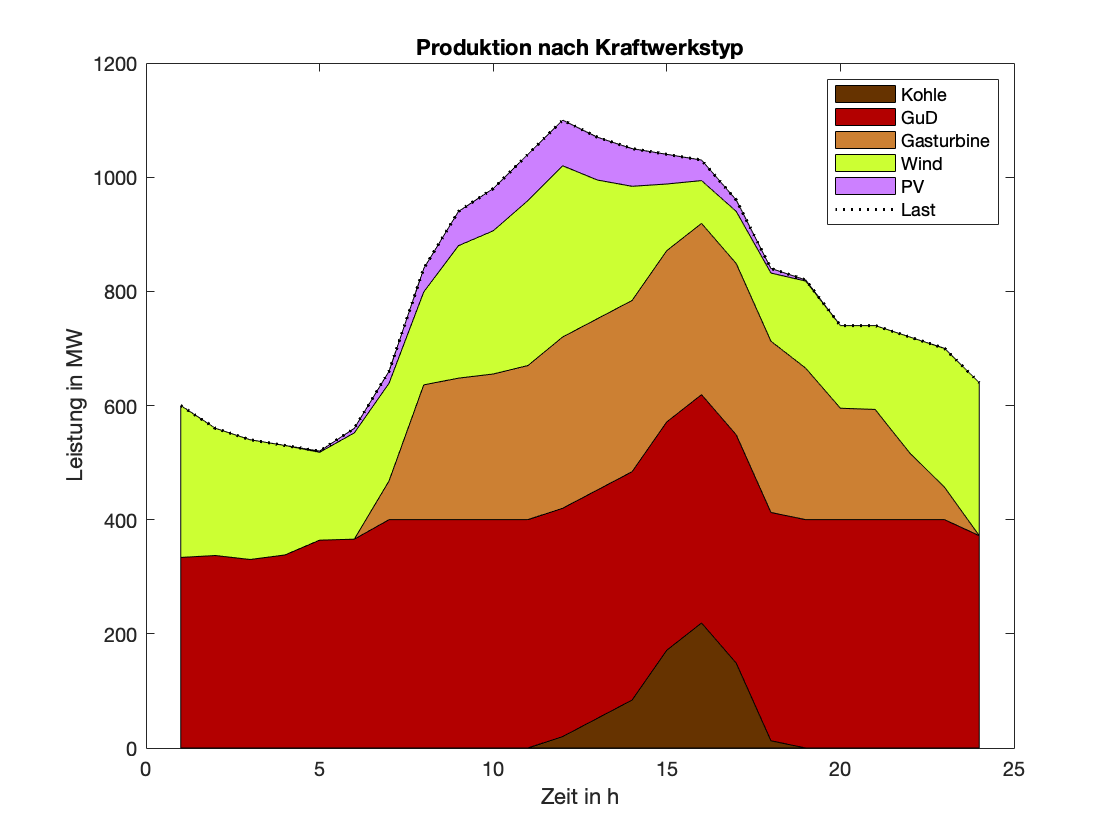
\includegraphics[width=1\linewidth]{graphics/Aufgabe_3_4_b_ohne_Speicher_Emission}
  \caption{ohne Speicher System}
  \label{fig:sfig2}
\end{subfigure}
\caption{Emissionsminimale Systeme}
\label{fig:1}
\end{figure}

\subsubsection{Gesamtkosten und -emissionen in Abhängigkeit des $CO_2$-Preises}
Aus der Abbildung a) ohne Speicher ist es ersichtlich, dass die Zertifikatkosten sich sehr diskret auswirken. Es gibt ungefähr zwei diskrete Sprünge wo sich die Gesamtemissionen drastisch ändern.Ab erstem Sprung ist KKW unwirtschaftlicher als GuD und ab zweitem Sprung KKW unwirtschaftlicher als GasKW. Bei der Abbildung b) mit Speicher gibt es mehrere Sprünge. Ab dem ersten Sprung wird das Pumpspeicherkraftwerk unwirtschaftlich, ab zweitem wird das KohleKW unwirtschaftlicher als GuD, ab drittem wird das KohleKW als GasKW unwirtschaftlicher und nach dem Sprung ähneln beide Optimierungsmodelle. 

\begin{figure}
\begin{subfigure}{.5\textwidth}
  \centering
  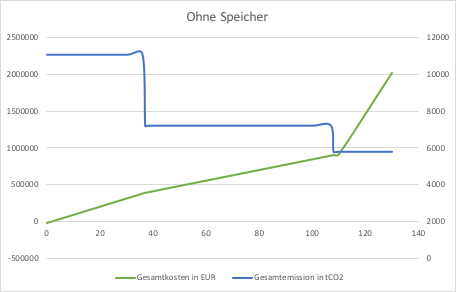
\includegraphics[width=0.9\linewidth]{graphics/Aufgabe_3_4_c_ohne_Speicher}
  \caption{ohne Speicher System}
  \label{fig:sfig2}
\end{subfigure}%
\begin{subfigure}{.5\textwidth}
  \centering
  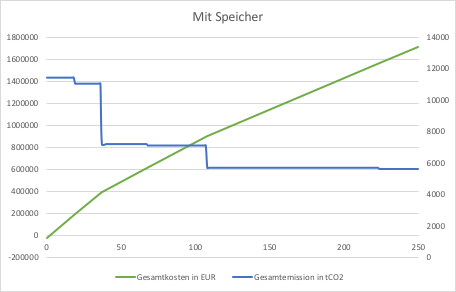
\includegraphics[width=0.9\linewidth]{graphics/Aufgabe_3_4_c_mit_Speicher}
  \caption{mit Speicher System}
  \label{fig:sfig1}
\end{subfigure}
\caption{Emissionsminimale Systeme}
\label{fig:1}
\end{figure}

\subsubsection{Preisinterpretation}
Ohne Speicher muss der $CO_2$-Preis mind. 108 EUR sein um auf die selben Emissionen wie bei dem emissionsminimalen Modell zu kommen, wobei wenn man den Speichertechnologie verwendet muss $CO_2$-Preis mindestens 224 EUR sein.

\newpage
\subsection{Emissionsschranken und Dualität}

\subsubsection{Lösung des Systems}
In dieser Aufgabe betrachten wir das kostenminimale System aus Aufgabe 3.2 (mit erneuerbarer Erzeugung, ohne Speicher) und verwenden die in der Aufgabe 3.4 ermittelten minimalen Emissionen (5793 t$CO_2$) als obere Emissionsschranke. Das heißt wir erhalten eine weitere Nebenbedinung, die besagt, dass die $CO_2$-Emissionen des System kleinergleich der Emissionsschranke sind!\\

Die Lösung für dieses System schaut wie folgt aus: 
\myfig{Aufgabe_3_5_a}
	{width=1.0\textwidth}
	{Emissionsschranke}
	{Emissionsschranke}
	{Emissionsschranke}
	{h!}

Die Gesamtkosten betragen 278333 EUR!
\subsubsection{Analyse der Schattenvariablen der Emissionsbeschränkung}
Um die Schattenvariablen der Emissionsbeschränkung zu analysieren wird wie in der Anleitung von Yalmip vorgegangen (siehe https://yalmip.github.io/command/dual/ ). Wir erhalten dabei einen Wert von 107,7586. Dieser Wert gibt uns an wie weit wir von unserer Nebenbedingung für die Emissionsbeschränkung abweichen können, unter Erhöhung der Zielfunktion (Systemkosten), um das duale Problem zu lösen. Dieser Wert entspricht genau dem in der Aufgabe 3.4)d) ermittelten $CO_2$-Preis! 

\subsubsection{Schlussfolgerung}
Zwischen der dualen Variable der Emissionsbeschränkung (Schattenpreis der Emission) und dem $CO_2$-Preis besteht ein indirekt proportionaler Zusammenhang, d.h. mit steigendem $CO_2$-Preis nimmt der Schattenpreis der Emission ab. Bei einem Wert von rund 108 EUR/t$CO_2$ verschwindet der Schattenpreis der Emission.

\newpage
\subsection{Erweiterung der Modellierung}

\subsubsection{Langfristige Grenzkosten}
Die langfristigen Grenzkosten im Gegensatz zu den kurzfristigen Grenzkosten bestehen noch aus dem fixen Anteil der Kosten, wie z.B  Kapitalkosten, betriebsbedingten Fixkosten und sonstigen Kosten die auf das Jahr bezogen werden.
Wenn man die langfristigen Grenzkosten in der Berechnung nimmt, so hängt der Einsatz
des Kraftwerks nicht mehr von den Rohstoffkosten ab, sondern ist nur noch von den jährlichen Anschaffungs- und
Betriebskosten abhängig.
Das könnte sich so auswirken, dass das in Anschaffung und Erhaltung günstigste
Kraftwerk, bis an seine Leistungsgrenze betrieben würde, bevor das nächst teurere zum Einsatz kommt.

\subsubsection{Ramp Up Costs}
Eine einfache Möglichkeit, Startkosten von Kraftwerken zu implementieren, ist eine Abfrage, mit Hilfe derer
überprüft wird ob ein Kraftwerk zu einem bestimmten Zeitpunkt Leistung liefern soll und zum vorherigen
Zeitpunkt keine Leistung lieferte.
Ist dies der Fall, werden Startkosten hinzugefügt, welche mit Hilfe einer binären Variable im Exponenten der
Startkostenvariable im Modell berücksichtigt werden können. Da das Modell nun einen Exponent hat, ist es nicht mehr möglich das Modell durch einen lineare Optimierung zu berechnen.
Um die maximalen Laständerungen zu berücksichtigen können Randbedingungen (Constraints) definiert werden, welche die Laständerung zum jetzigen Zeitpunkt mit dem vorherigen vergleichen.

\appendix


\newpage
%auskommentieren wenn notwendig:

\listoffigures   
\listoftables
%\printbibliography

\end{document}